%%  Figures of methodology


\begin{figure}
	\centering
	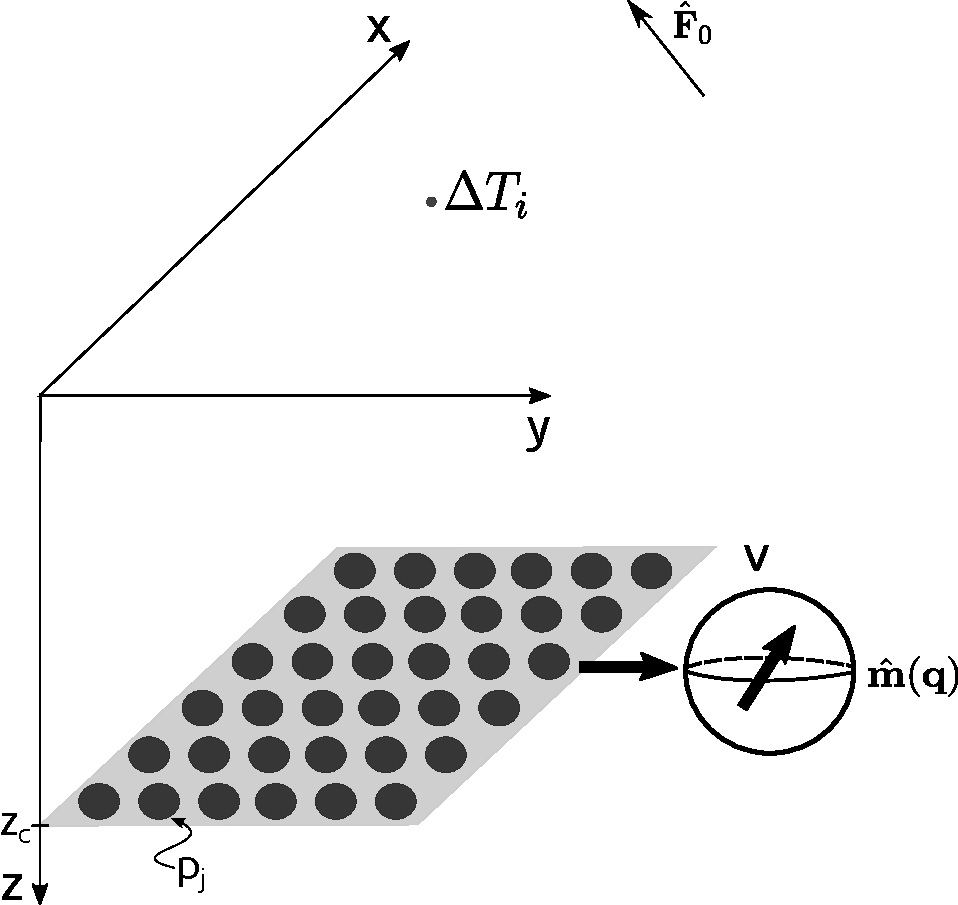
\includegraphics[width=0.7\textwidth]{Fig/eqlayer_figure.pdf}
	\caption{Schematic representation of an equivalent layer. The layer is positioned over the horizontal plane at a depth of $z=z_c$. $\Delta T_i =  f_i (\mathbf{s})$ is the predicted total-field anomaly at the point $(x_i,y_i,z_i)$ produced by the set of $M$ equivalent sources (black dots). Each source is located at the point $(x_j,y_j,z_c)$, $j = 1,\hdots, M$, and represented by a dipole with unity volume $\upsilon$ with magnetization direction $\hat{\mathbf{m}}(\mathbf{q})$ and magnetic moment $p_j$.    }
	\label{fig:eqlayer_figure}
\end{figure}


%% Figures synthetic tests

\begin{figure}
	\centering
	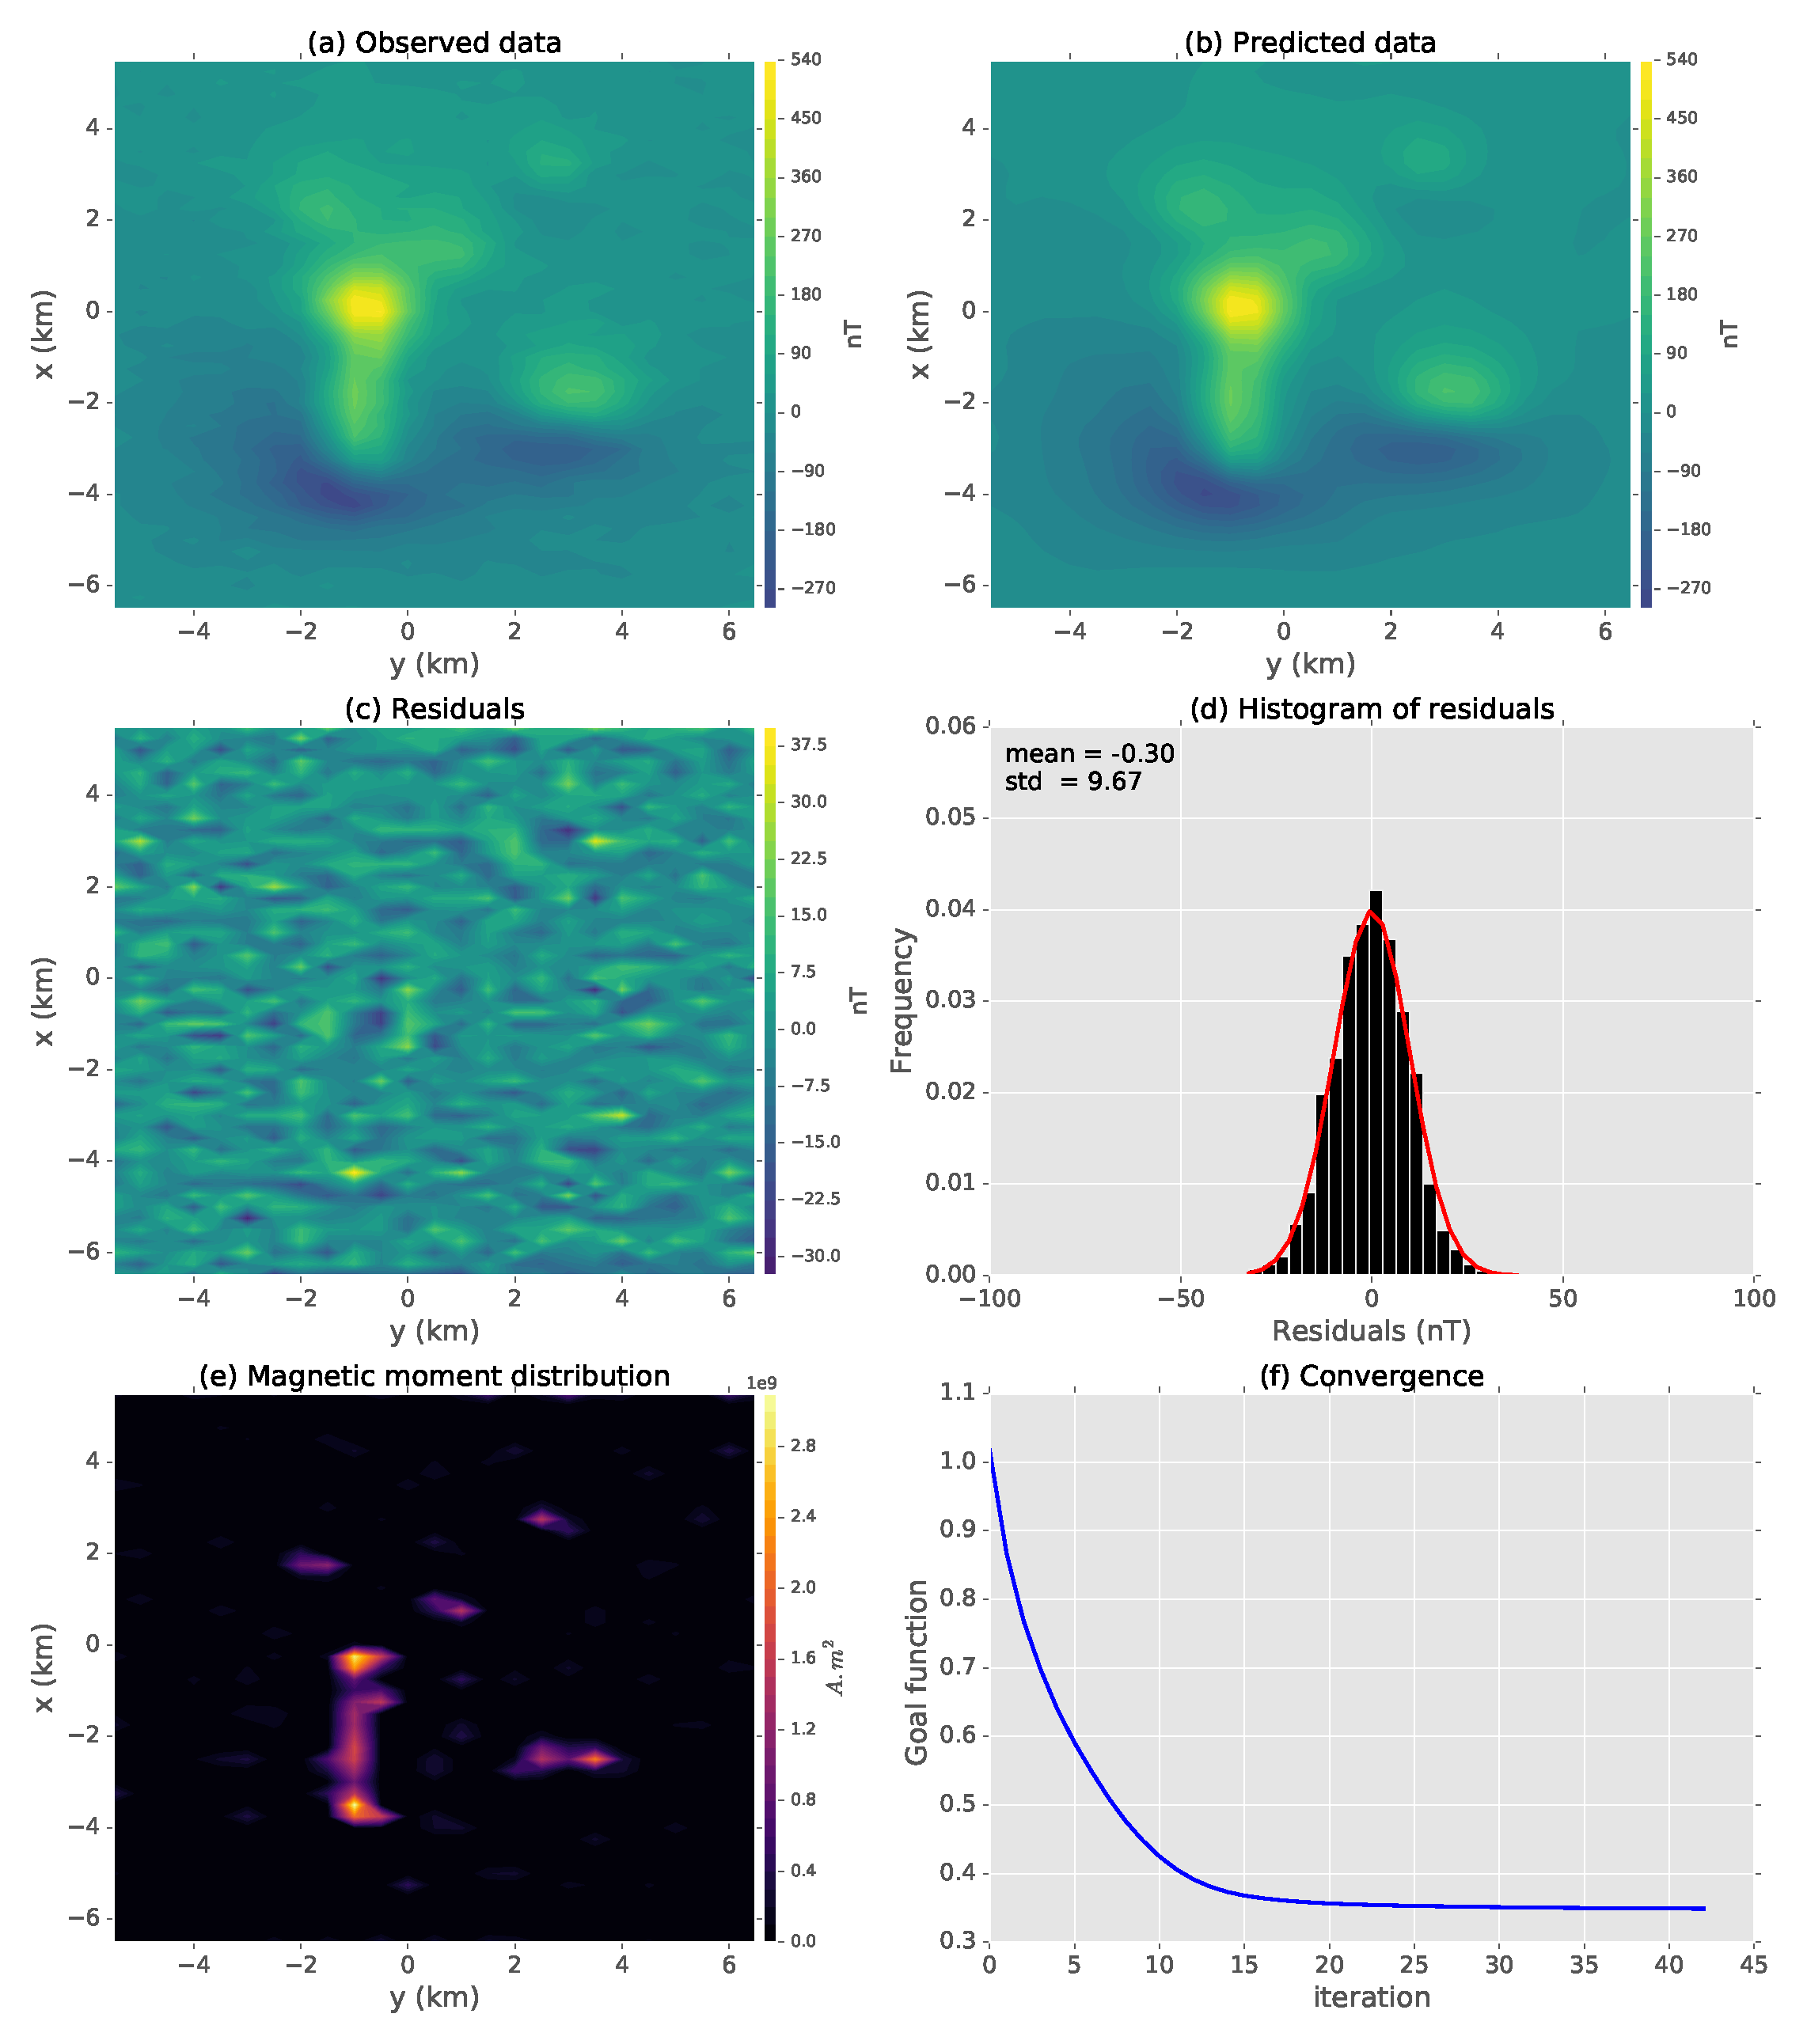
\includegraphics[width=0.85\textwidth]{Fig/unidir_test/results_compiled_LM_NNLS_magRM.eps}
	\caption{Application to synthetic data for multiple sources with unidirectional magnetization. (a) Noise-corrupted total-field anomaly. (b) Predicted data produced by equivalent layer. (c) Difference between the data shown in panels a and b. (d) Histogram of residuals. (e) All-positive magnetic-moment distribution. (f) Goal function value (equation \ref{eq:positivity_goal_function}a) per iteration showing the convergence.}
	\label{fig:unidir_test}
\end{figure}

\begin{figure}
	\centering
	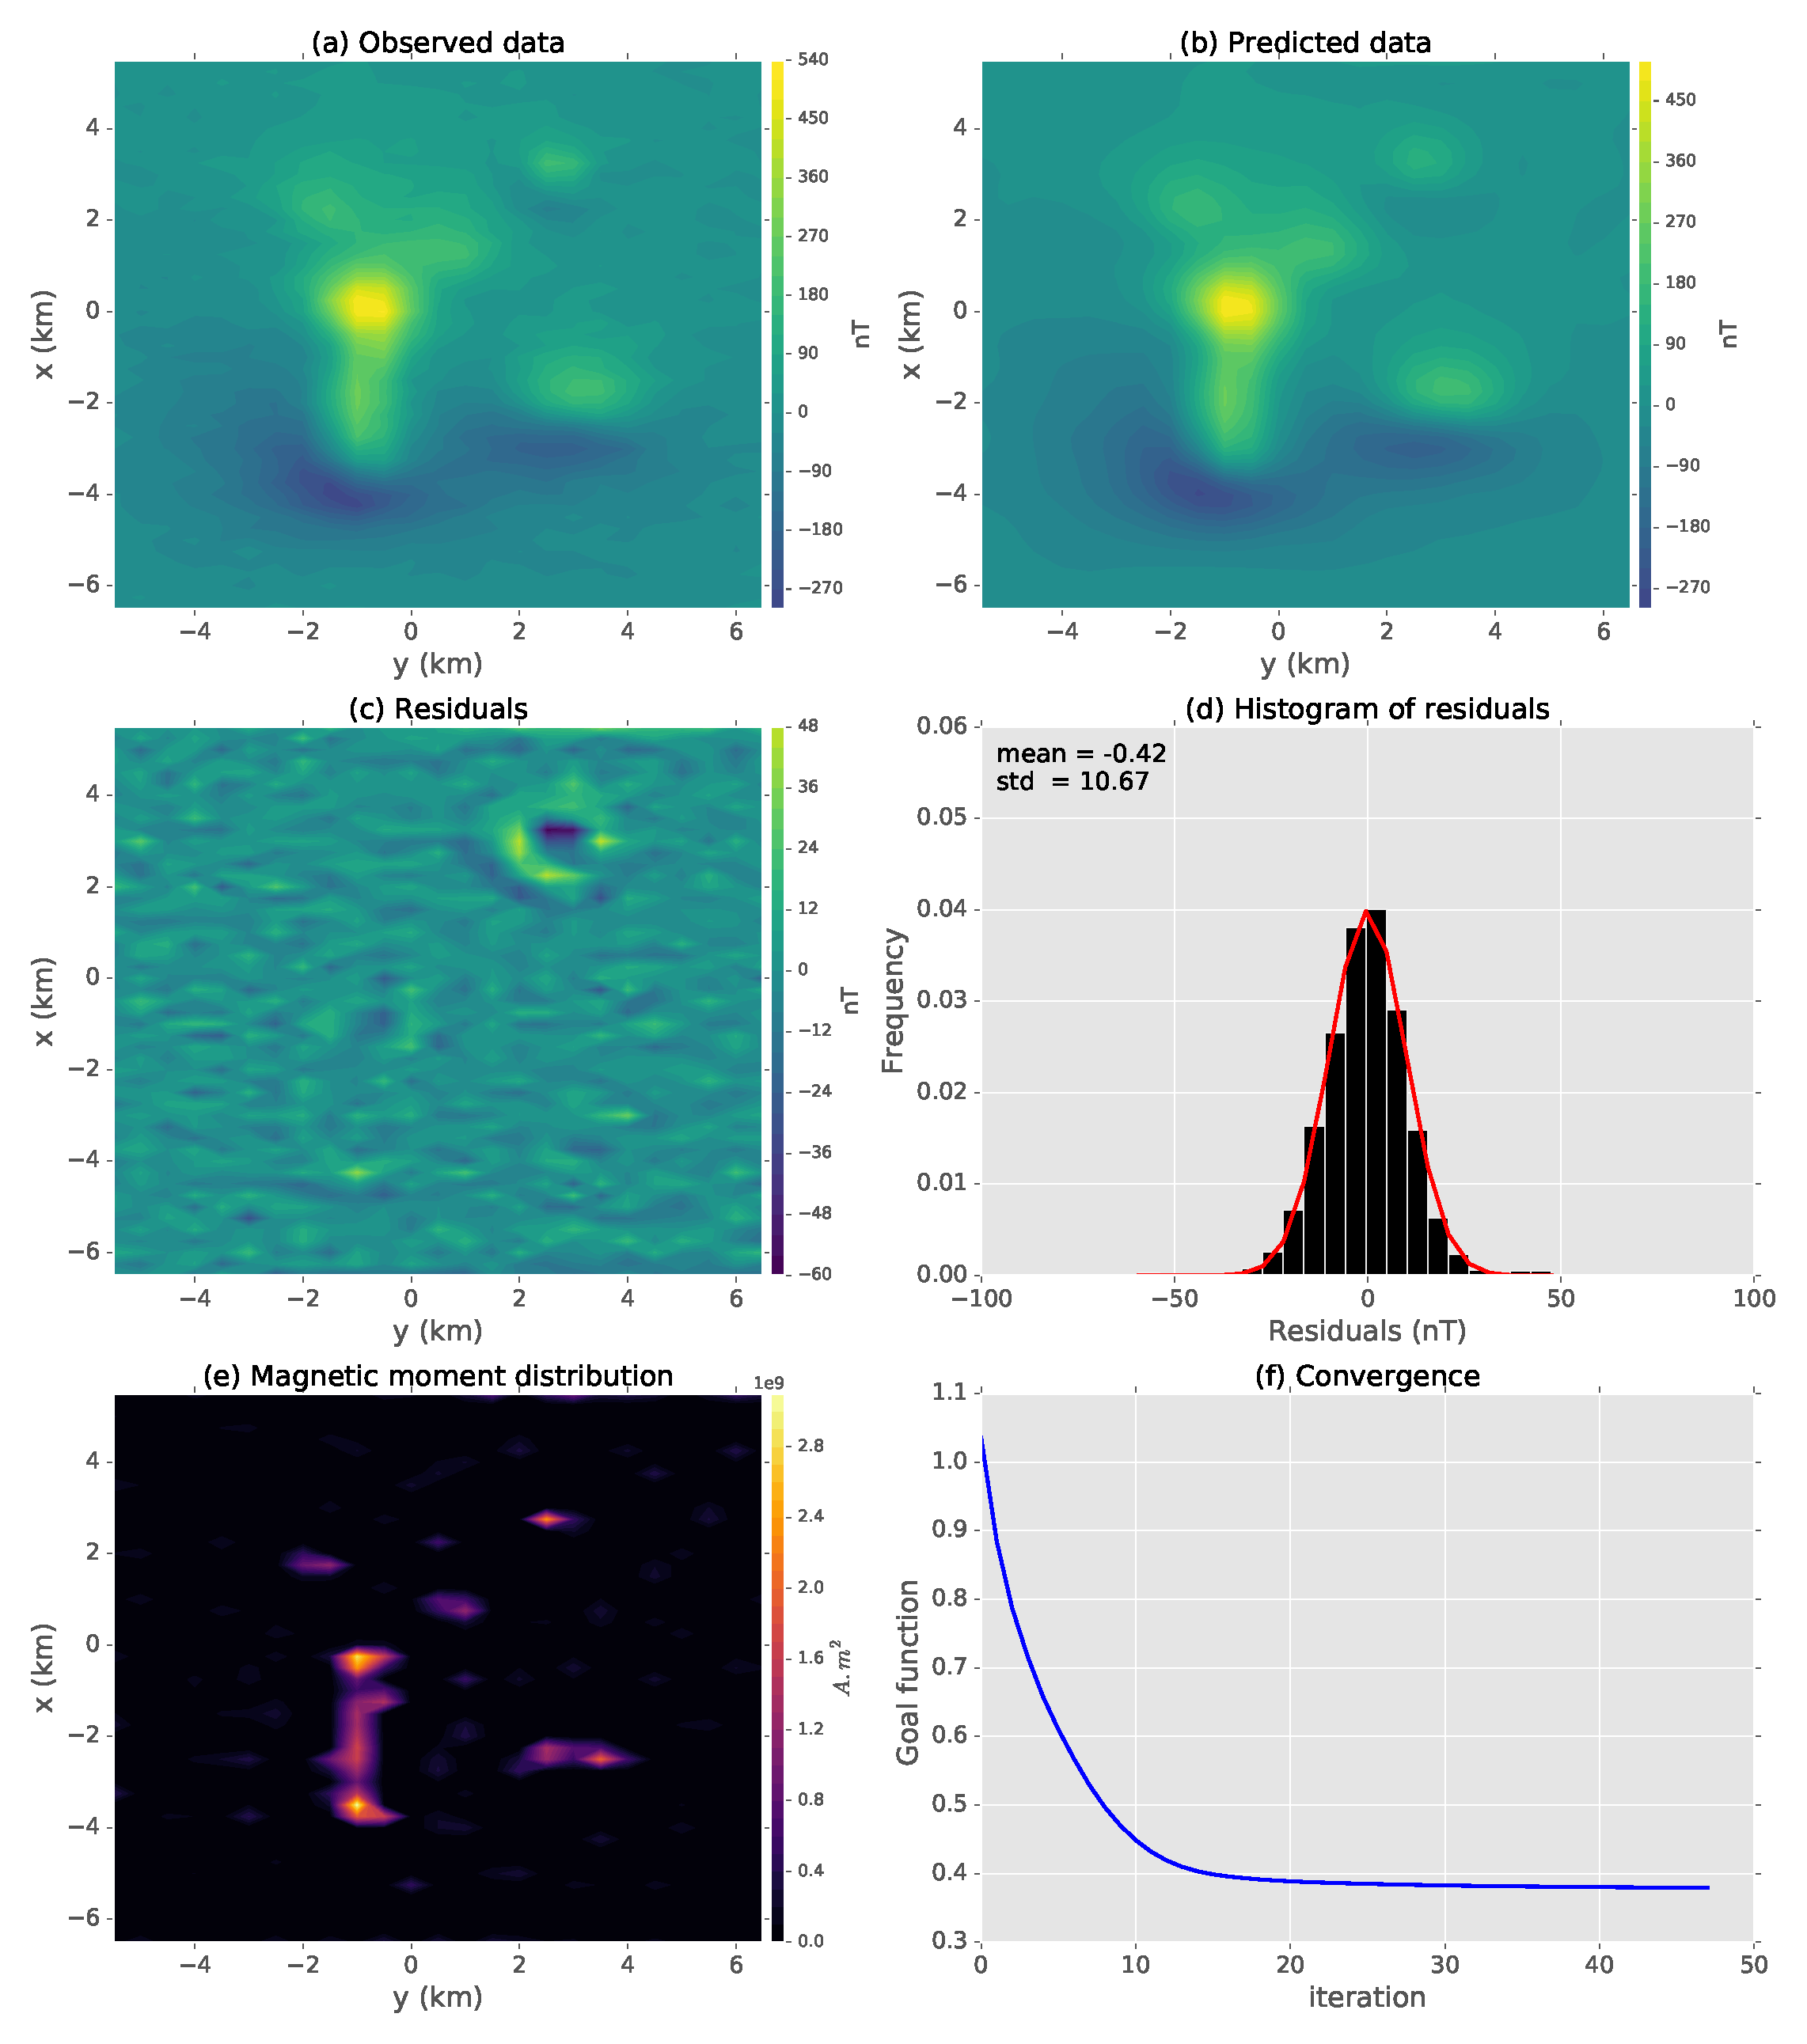
\includegraphics[width=0.85\textwidth]{Fig/unidir_shallow_test/results_compiled_LM_NNLS_magRM.eps}
	\caption{Multiple synthetic sources with a shallow-seated body under unidirectional magnetization . (a) Noise-corrupted total-field anomaly. (b) Predicted data produced by equivalent layer. (c) Difference between the data shown in panels a and b. (d) Histogram of residuals. (e) All-positive magnetic-moment distribution. (f) Goal function value (equation \ref{eq:positivity_goal_function}a) per iteration showing the convergence.}
	\label{fig:unidir_shallow_test}
\end{figure}

\begin{figure}
	\centering
	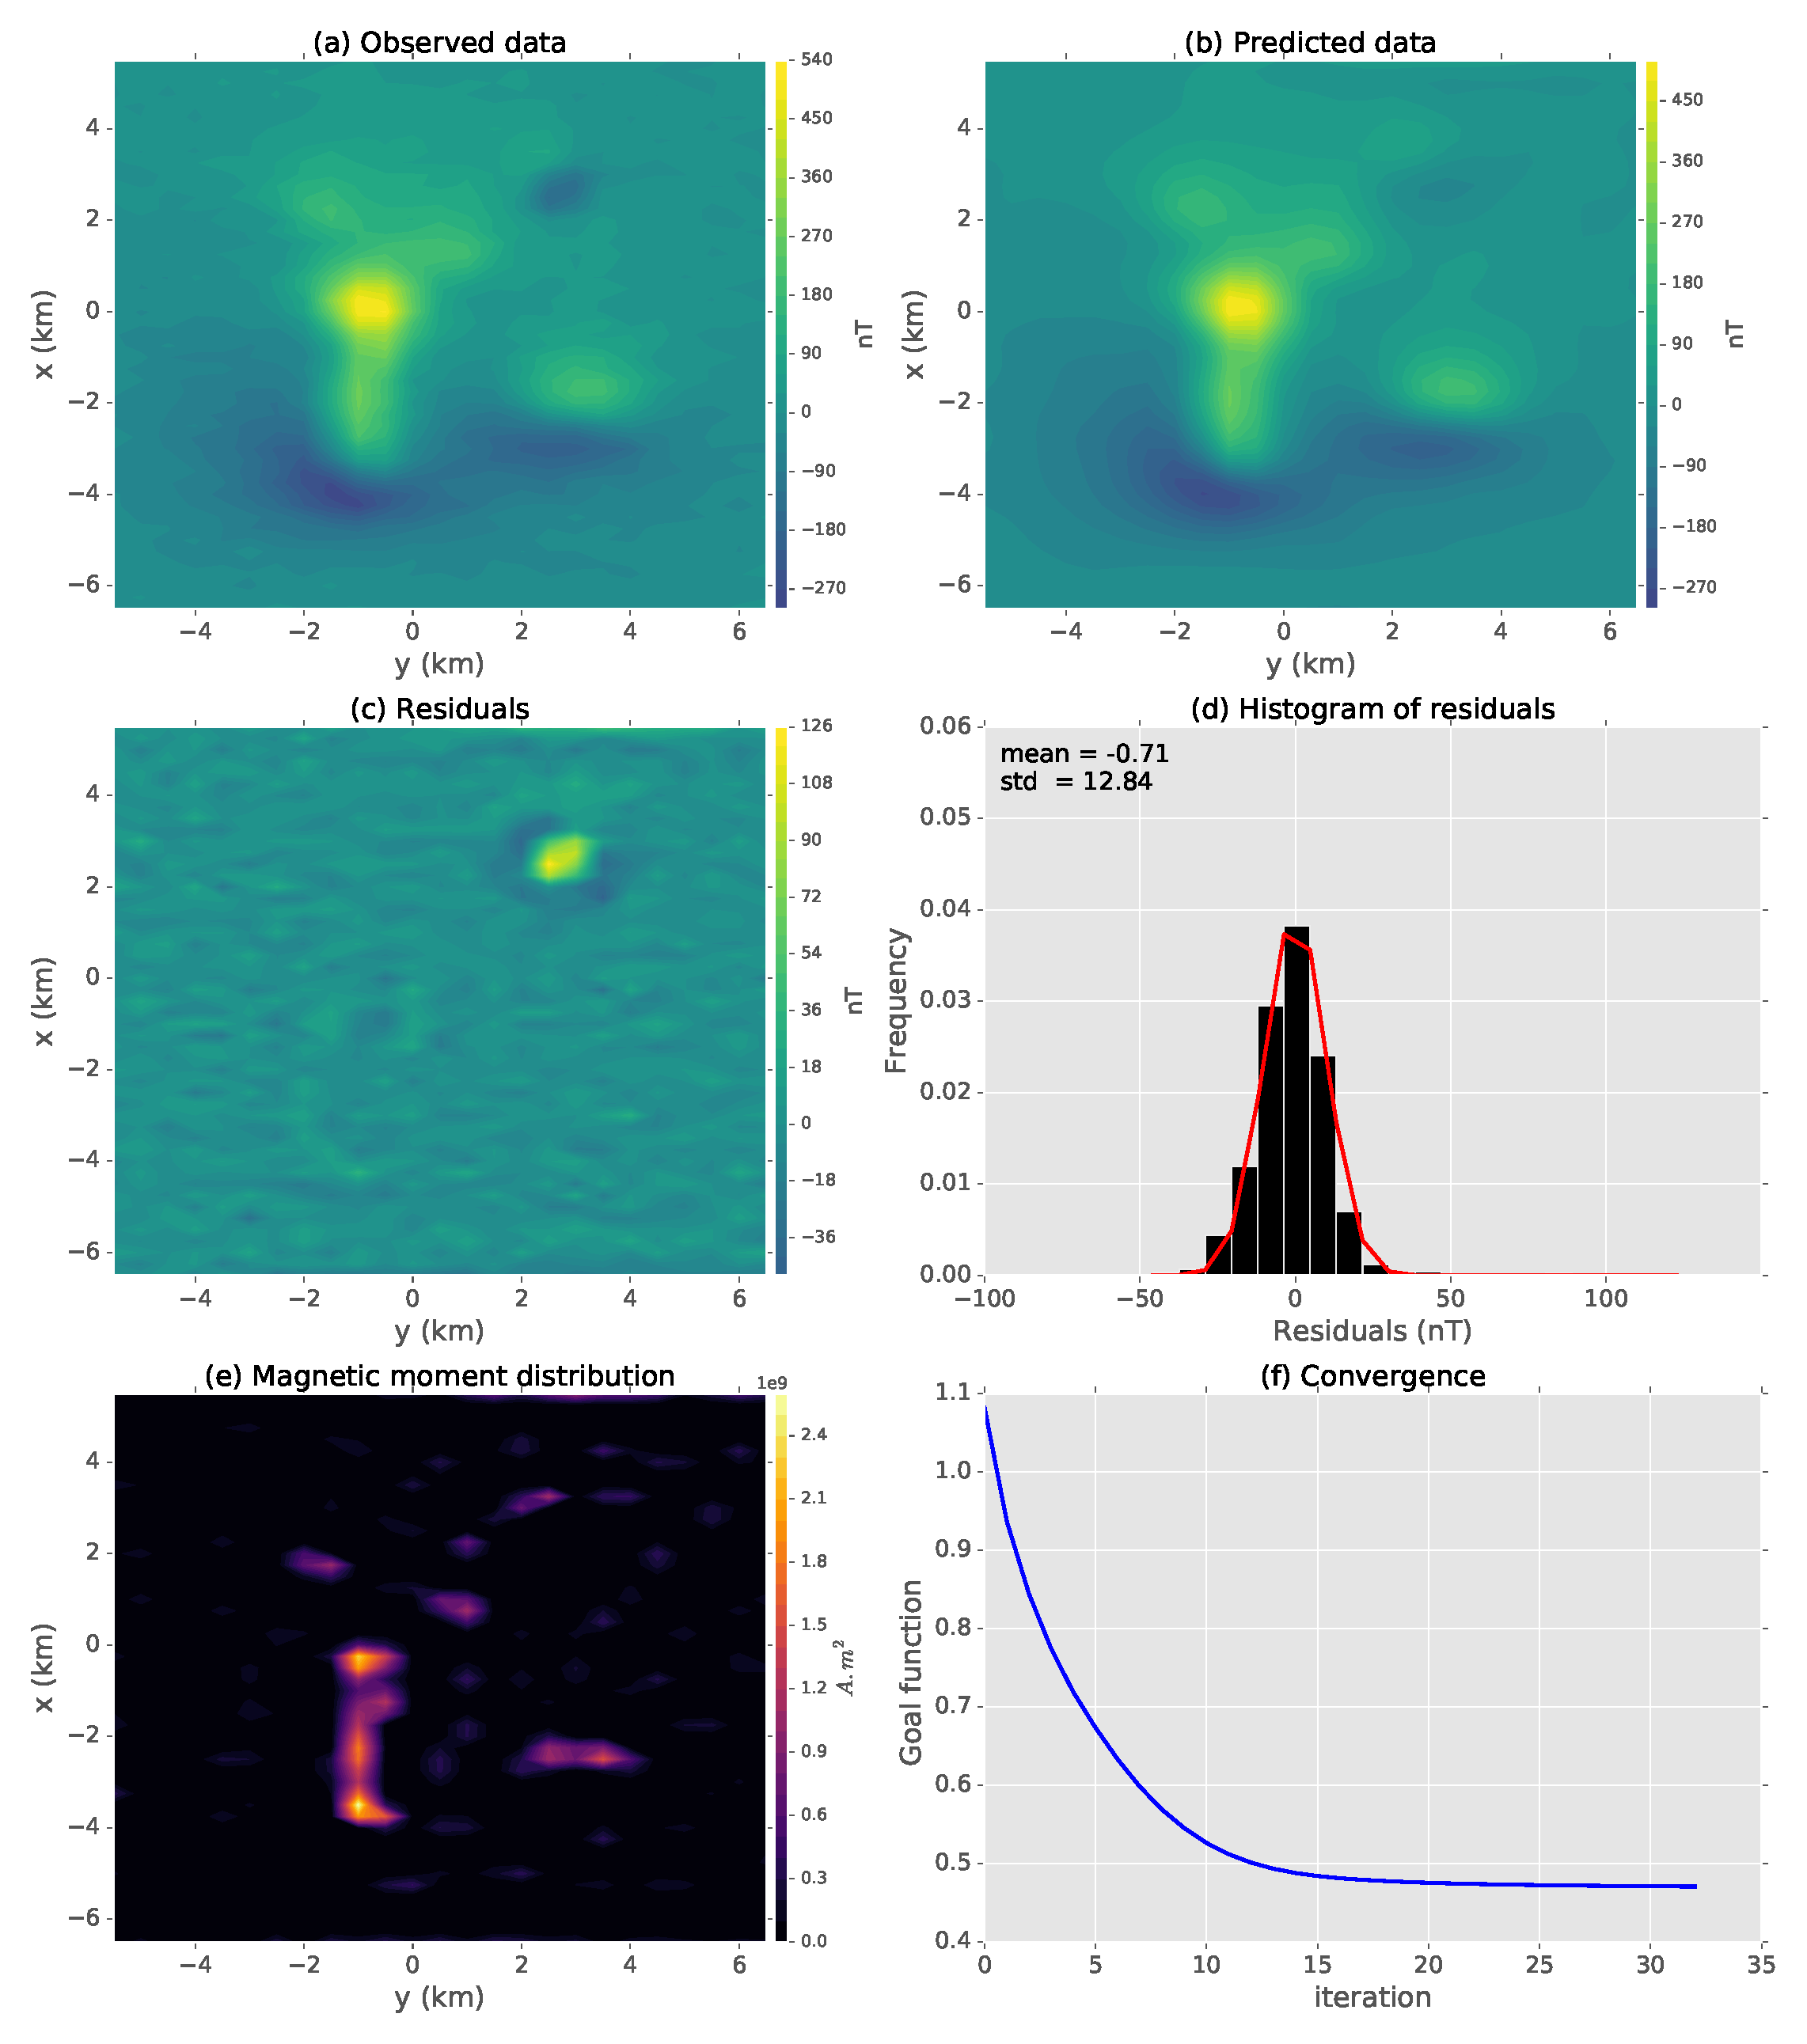
\includegraphics[width=0.85\textwidth]{Fig/unidir_shallow_diff_test/results_compiled_LM_NNLS_magRM.eps}
	\caption{Multiple synthetic sources with a shallow-seated body under different magnetization directions. (a) Noise-corrupted total-field anomaly. (b) Predicted data produced by equivalent layer. (c) Difference between the data shown in panels a and b. (d) Histogram of residuals. (e) All-positive magnetic-moment distribution. (f) Goal function value (equation \ref{eq:positivity_goal_function}a) per iteration showing the convergence.}
	\label{fig:unidir_shallow_diff_test}
\end{figure}

%% Real data application 
\begin{figure}
	\centering
	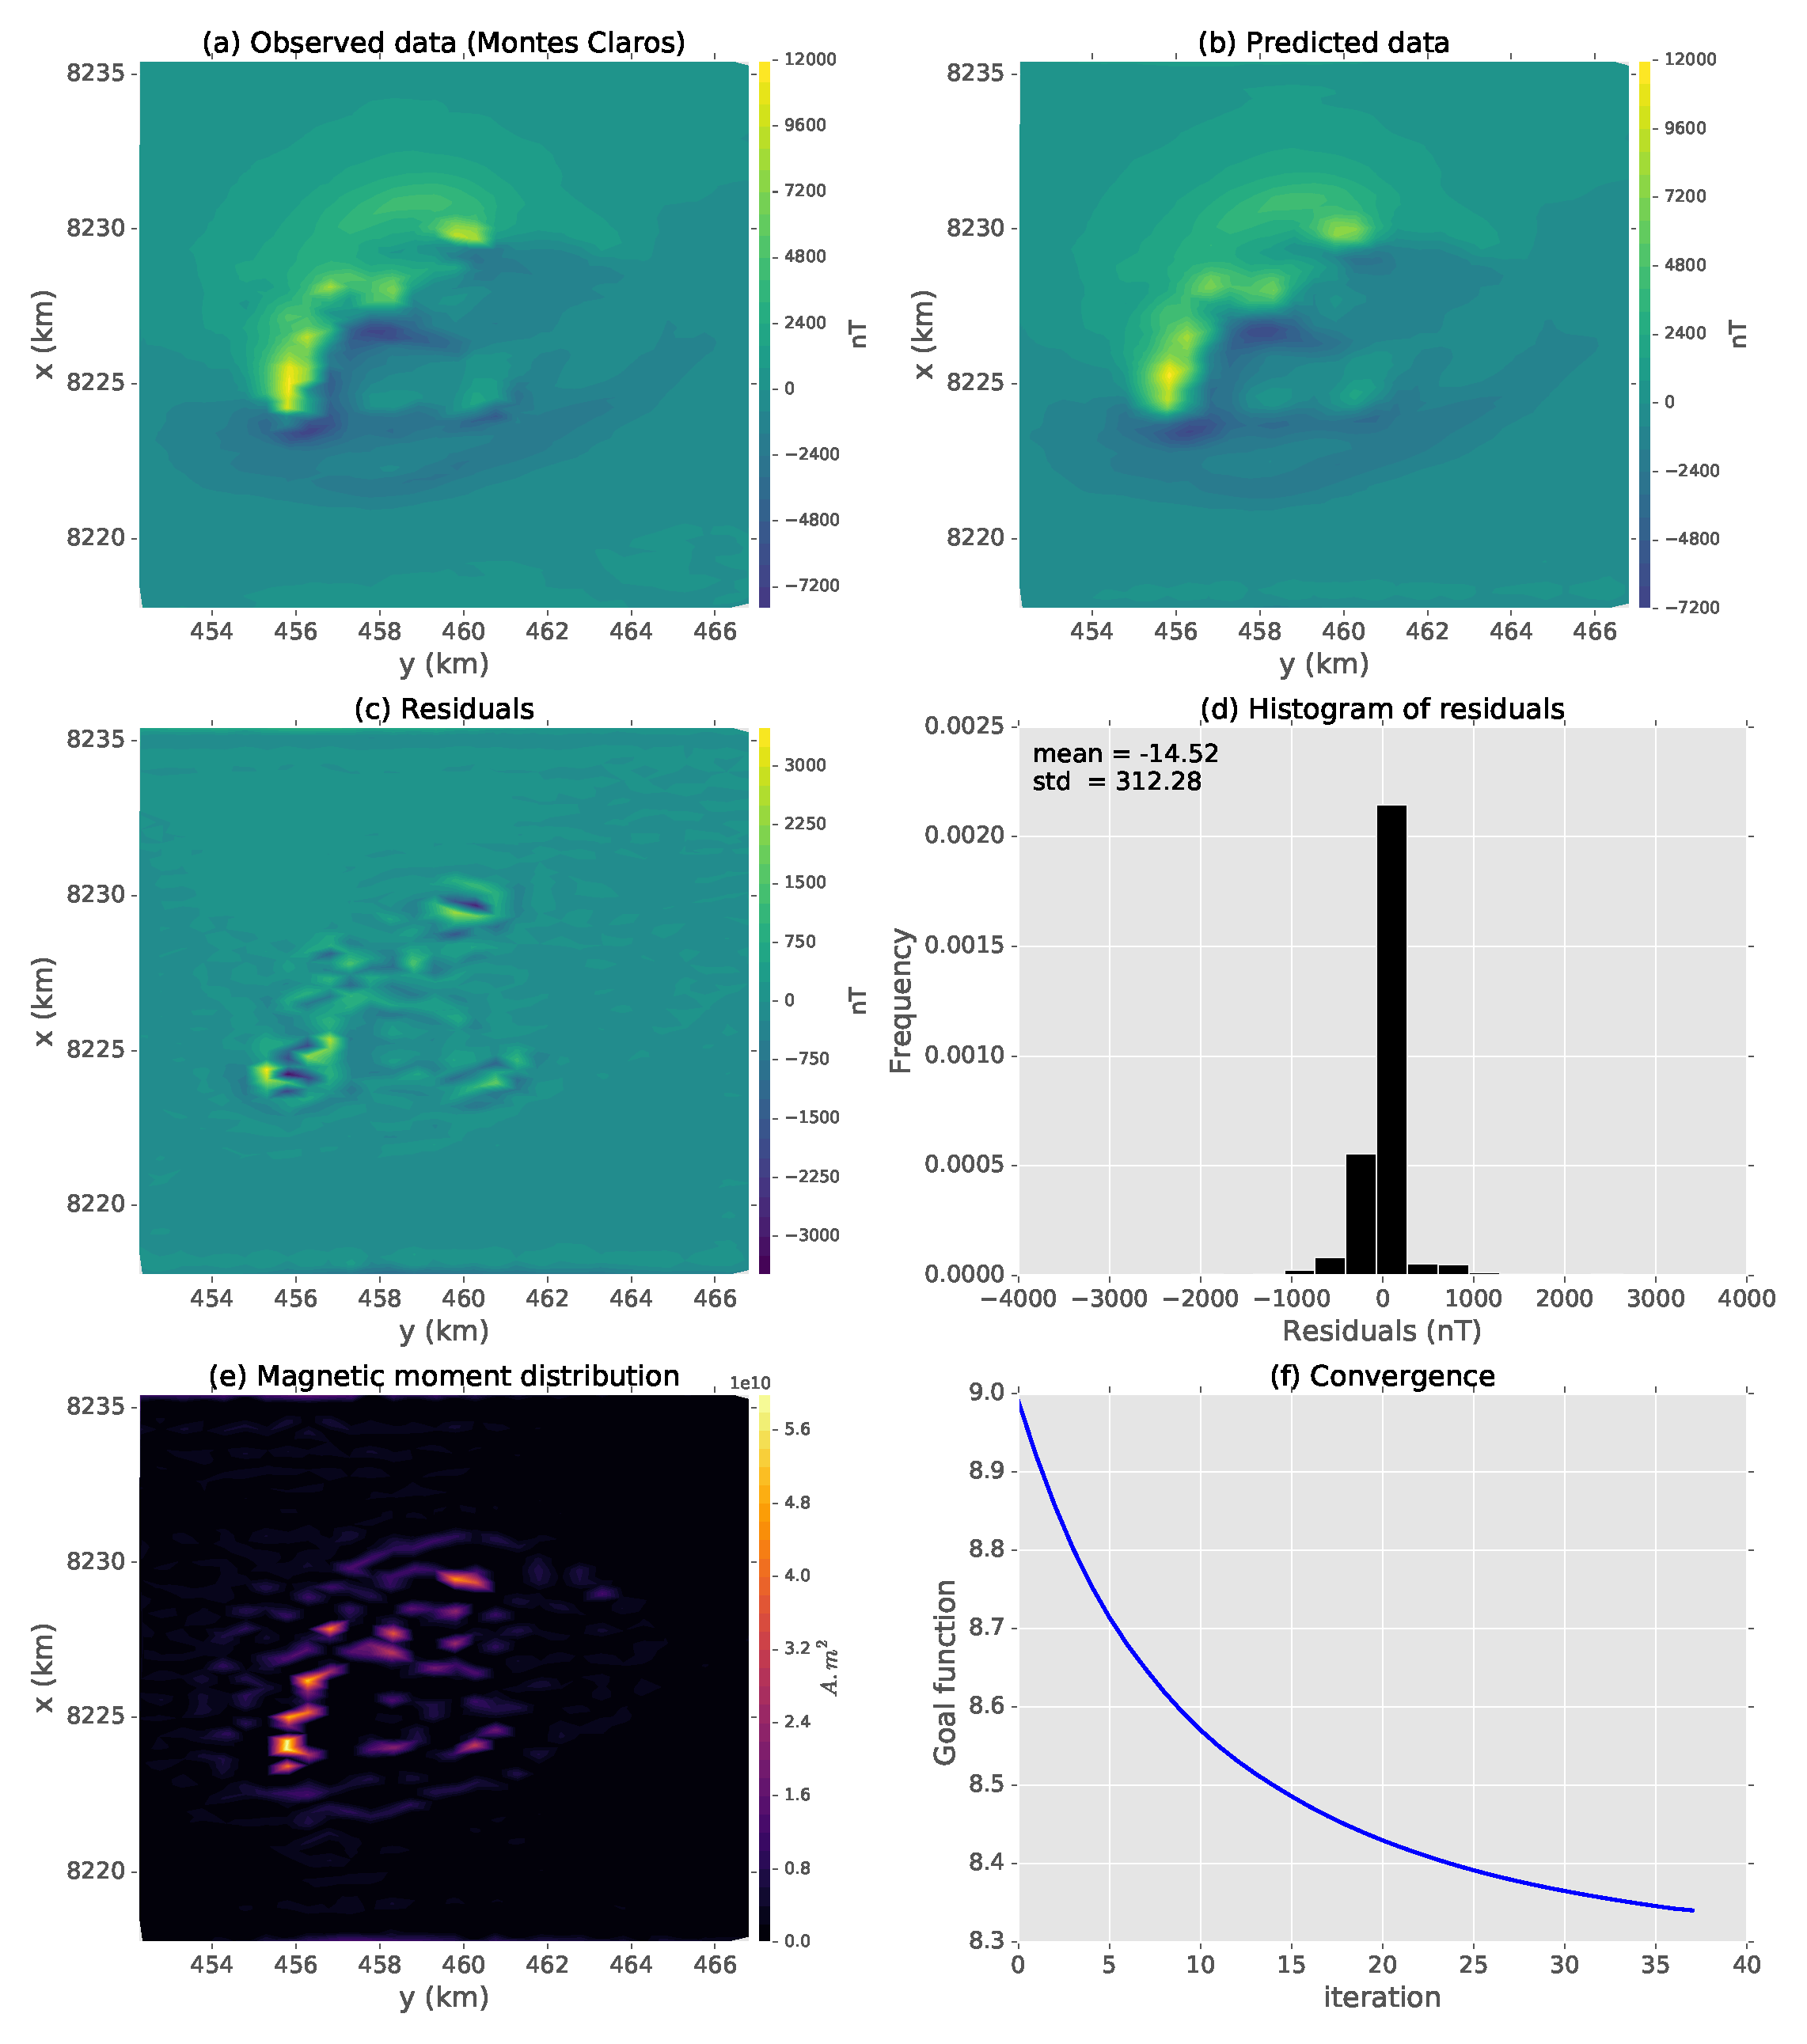
\includegraphics[width=0.85\textwidth]{Fig/field_data_montes_claros/montes_claros_compiled_LM_NNLS_magRM.eps}
	\caption{Application to field data from alkaline complex of Montes Claros (Brazil). (a) Observed total-field anomaly. (b) Predicted data produced by equivalent layer. (c) Difference between the data shown in panels a and b. (d) Histogram of residuals. (e) All-positive magnetic-moment distribution. (f) Goal function value (equation \ref{eq:positivity_goal_function}a) per iteration showing the convergence.}
	\label{fig:mc_data_application}
\end{figure}

\begin{figure}
	\centering
	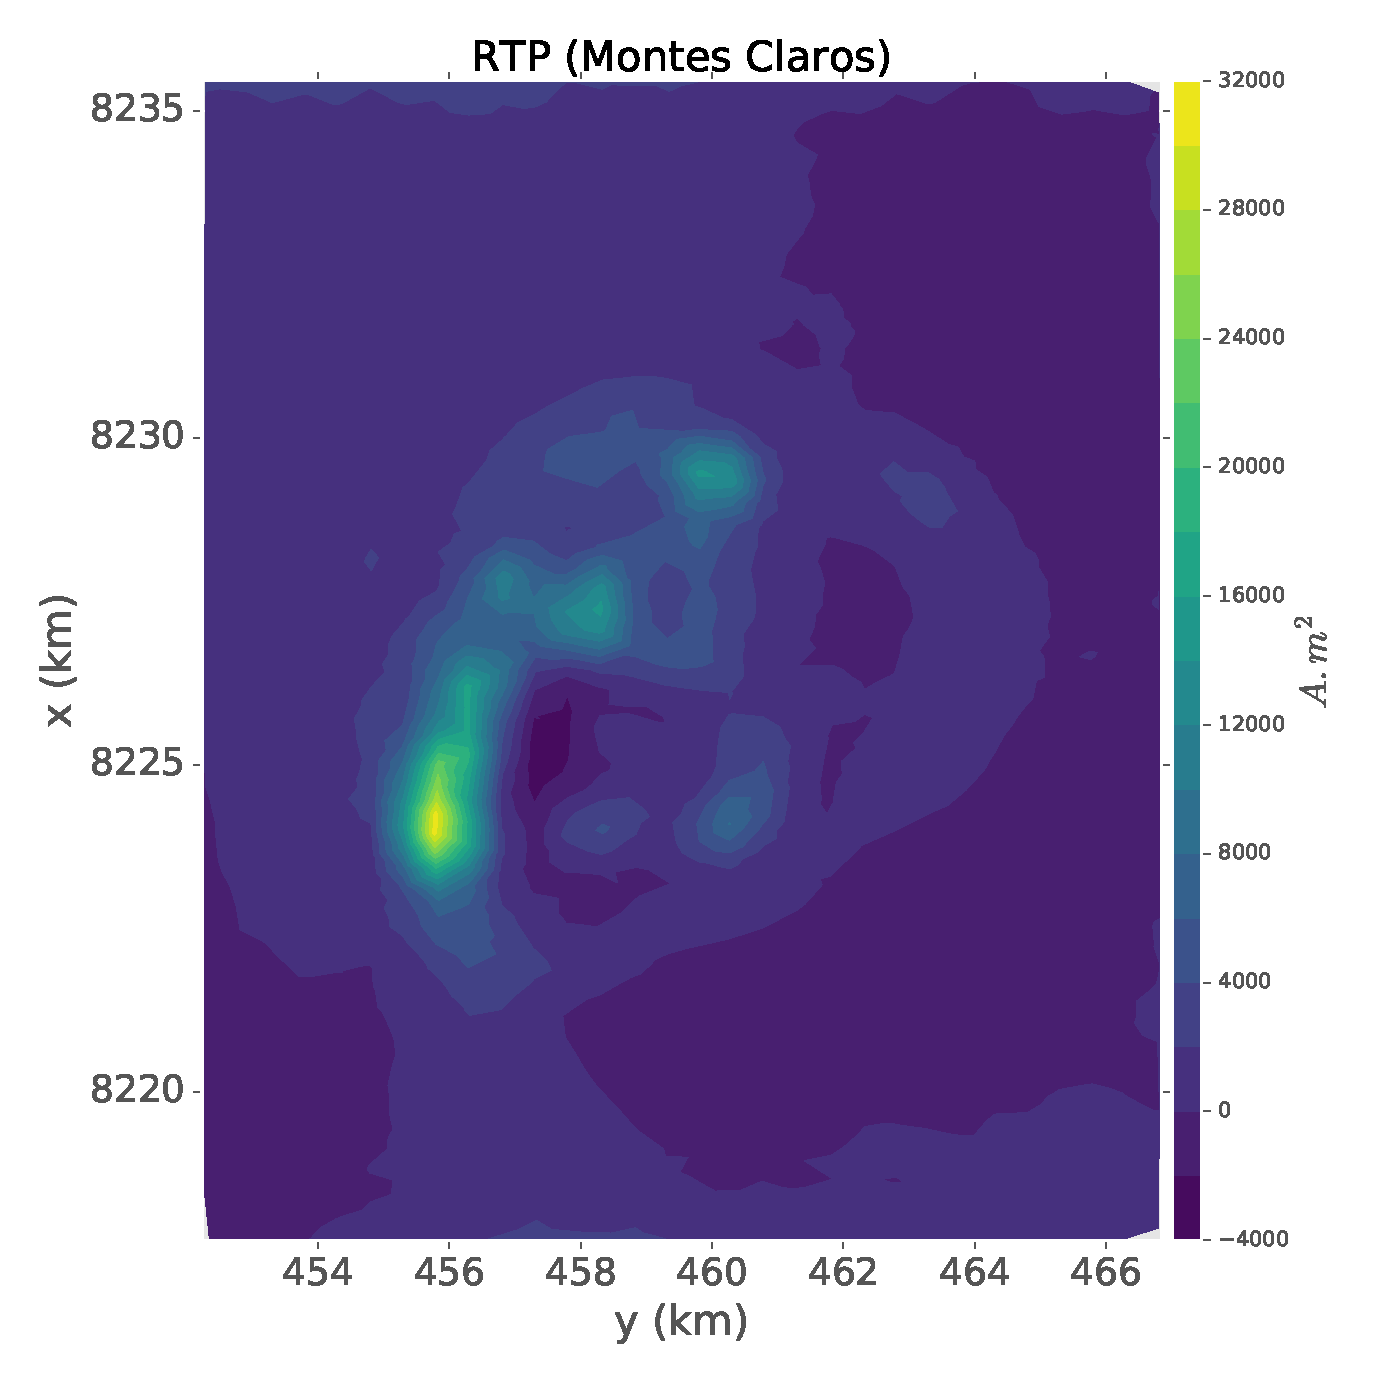
\includegraphics[width=0.75\textwidth]{Fig/field_data_montes_claros/RTP_data_montes_claros.eps}
	\caption{Application to field data from alkaline complex of Montes Claros (Brazil). RTP anomaly computed by using the estimated magnetization distribution shown in figure \ref{fig:mc_data_application}e.}
	\label{fig:rtp_mc_data}
\end{figure}

%% Appendix 

\begin{figure}
	\centering
	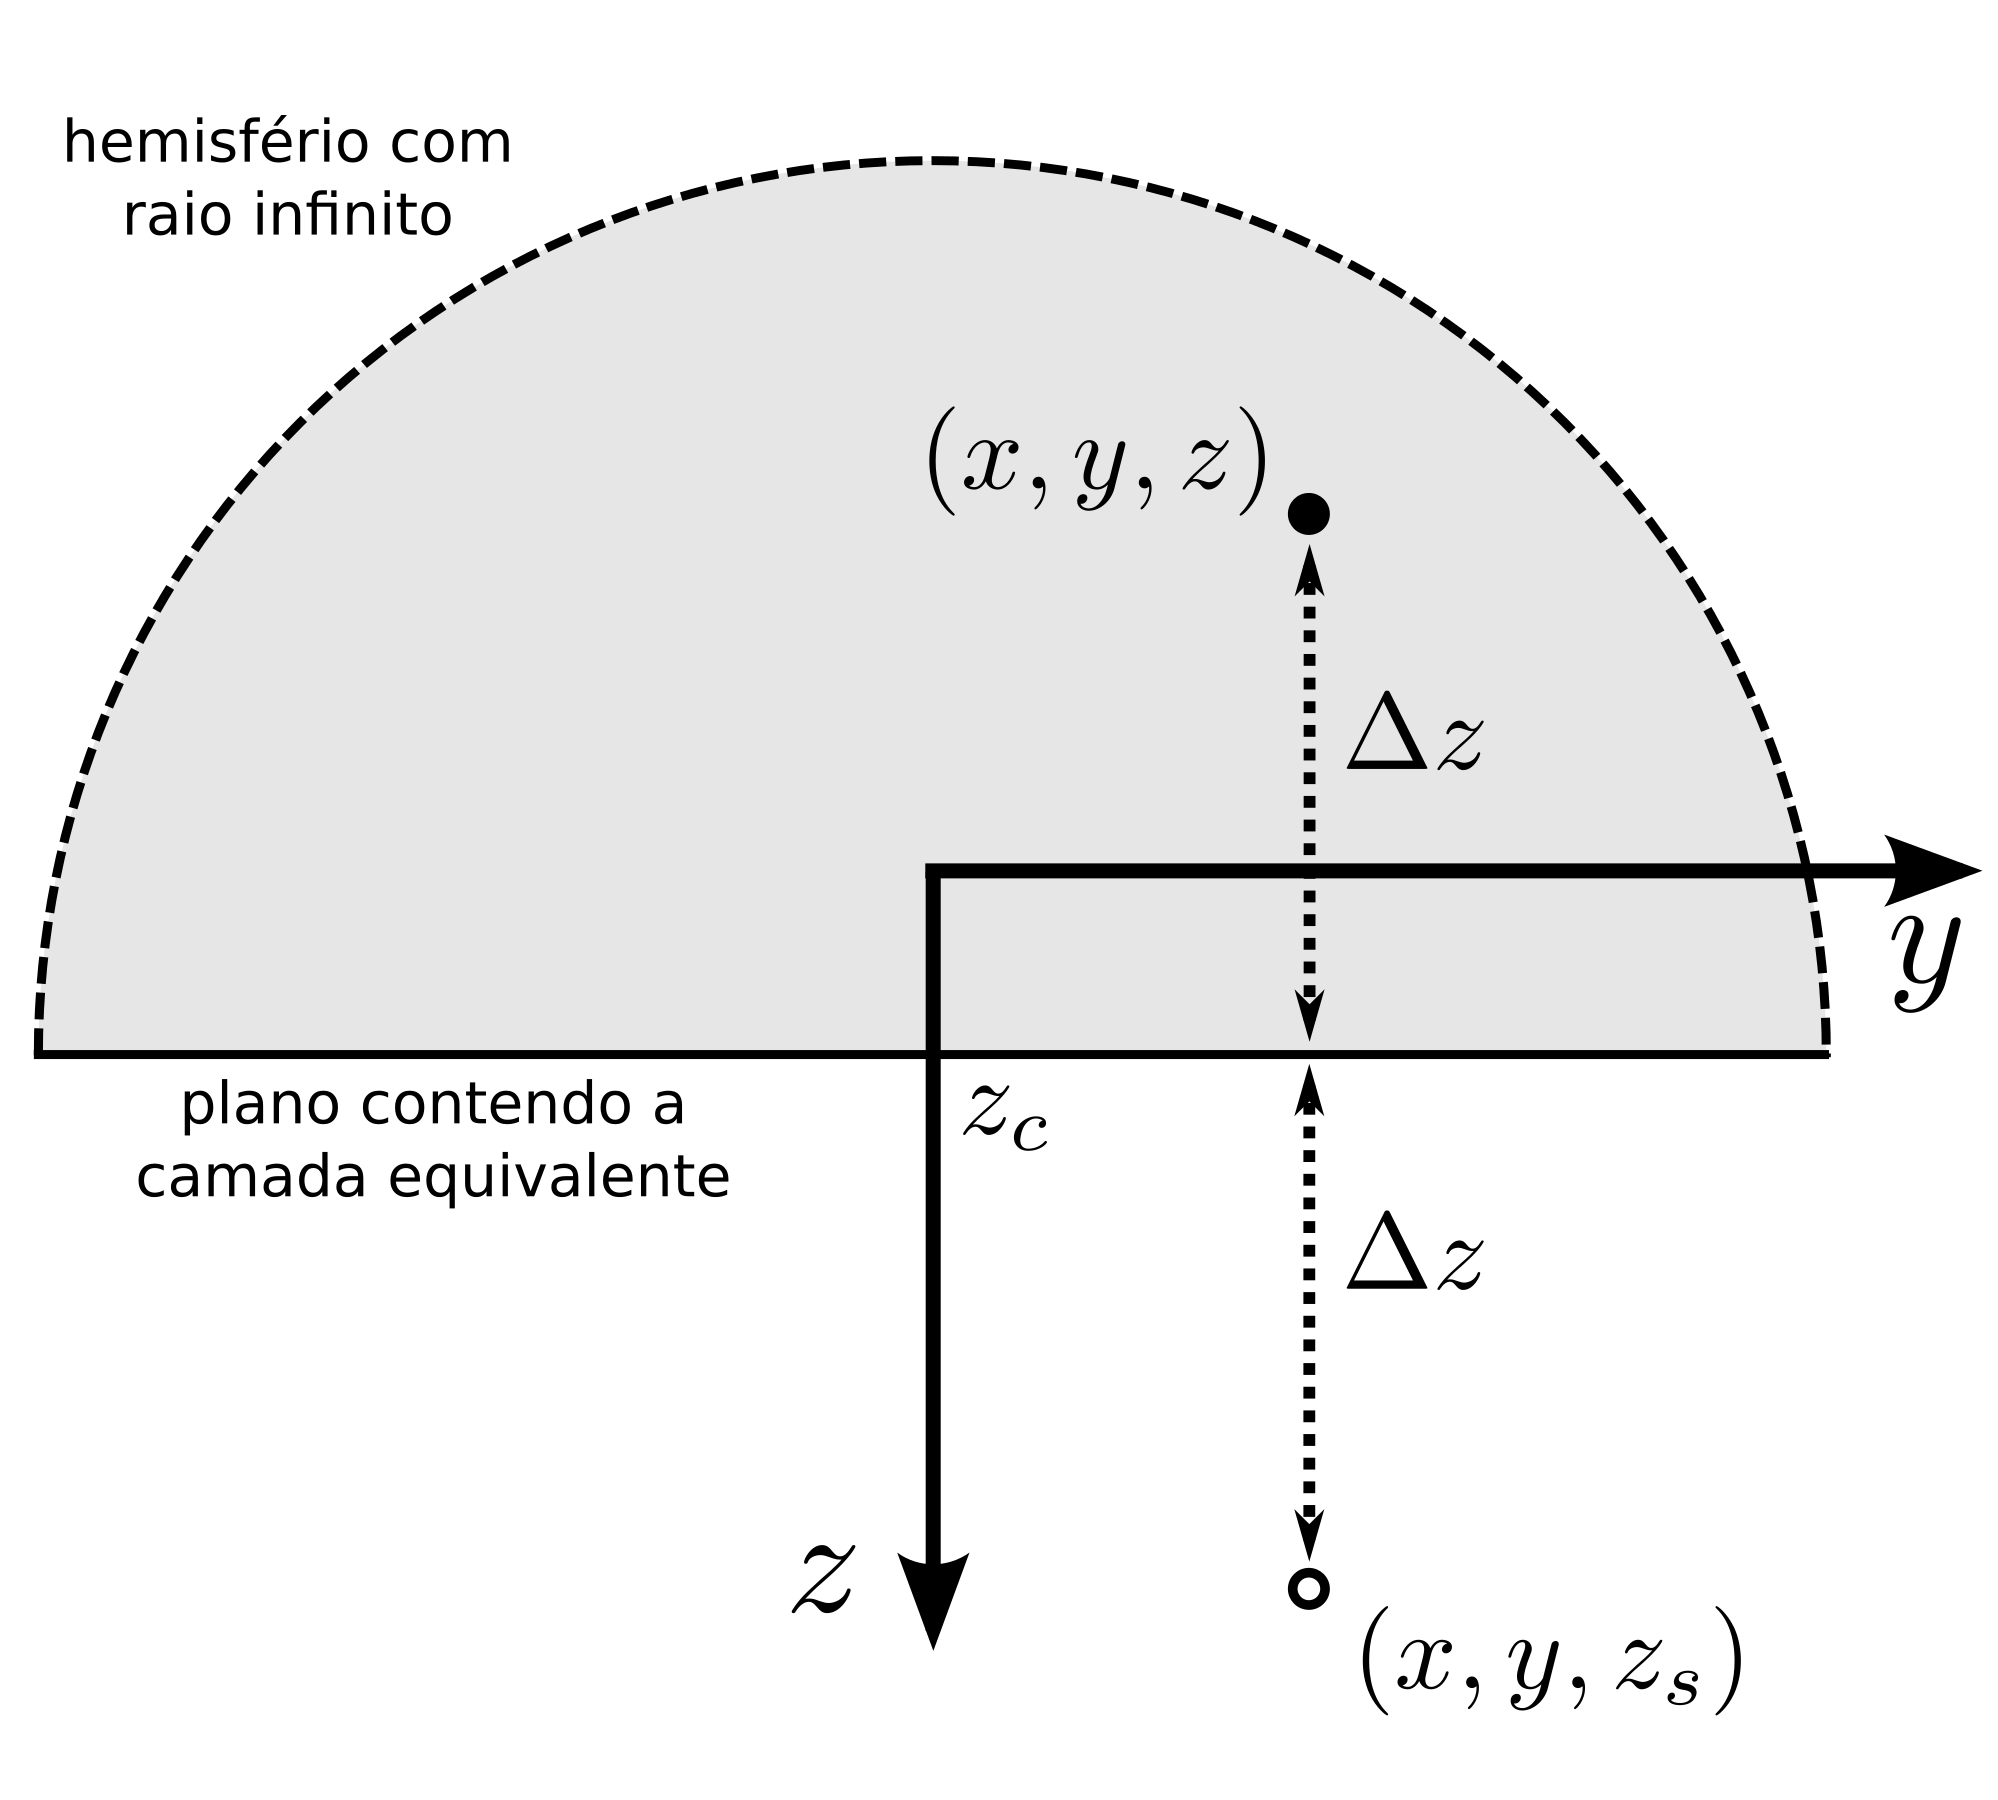
\includegraphics[width=0.75\textwidth]{Fig/surface_Green}
	\caption{2D representation of the surface used for applying the Green's 
	identities. The surface is formed by a hemisphere (dashed line) with infinite
	radius and the plane $z = z_{c}$ containing the equivalent layer. 
	The points $(x, y, z)$ (black dot) and $(x, y, z_{s})$ (white dot) are 
	symmetrically positioned with respect to the plane $z = z_{c}$ and are
	defined by $z = z_{c} - \Delta z$ and $z = z_{c} + \Delta z$, respectively.}
	\label{fig:surface_Green}
\end{figure}